\documentclass[tikz,border=6pt]{standalone}
\usepackage{tikz}
\usetikzlibrary{decorations.pathmorphing} % 画波浪线可选

\begin{document}
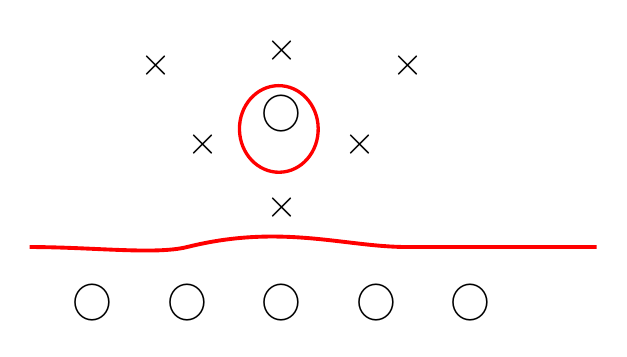
\begin{tikzpicture}[x=1cm,y=1cm,
    every node/.style={font=\bfseries\Large}]

% ==== 上半部分：X 们 + 被圈的 $\bigcirc$ ====
% 摆几个 X（坐标可按需改）
\node at (-1.6, 2.8) {$\times$};
\node at ( 0.0, 3.0) {$\times$};
\node at ( 1.6, 2.8) {$\times$};
\node at (-1.0, 1.8) {$\times$};
\node at ( 1.0, 1.8) {$\times$};
\node at ( 0.0, 1.0) {$\times$};

% 中间被圈的 $\bigcirc$
\node (Ocenter) at (0,2.2) {$\bigcirc$};

% 红色椭圆圈选
\draw[red, line width=1.2pt, rotate=1]
      (0,2) ellipse [x radius=0.5cm, y radius=0.55cm];


% ==== 中间的红色波浪分隔线 ====
% 用平滑样条画一条波浪线
\draw[red, line width=1.4pt]
  (-3.2,0.5) .. controls (-2.4,0.5) and (-1.6,0.4) ..
  (-1.2,0.5) .. controls (0.0,0.8) and (0.8,0.5) ..
  (1.6,0.5) .. controls (2.4,0.5) and (3.2,0.5) .. (4.0,0.5);

% 也可以用装饰器画更“波浪”的线（把上面注释掉，启用下面两行）：
% \draw[red, line width=1.4pt, decorate, decoration={snake, amplitude=1.5mm, segment length=8mm}]
%   (-3.2,0.8) -- (4.0,0.8);

% ==== 下半部分：一排 $\bigcirc$ ====
\node at (-2.4,-0.2) {$\bigcirc$};
\node at (-1.2,-0.2) {$\bigcirc$};
\node at ( 0.0,-0.2) {$\bigcirc$};
\node at ( 1.2,-0.2) {$\bigcirc$};
\node at ( 2.4,-0.2) {$\bigcirc$};


\end{tikzpicture}
\end{document}